
\documentclass{article}
\usepackage{polski}
\usepackage[utf8]{inputenc}
\usepackage{graphicx}

\begin{document}

\title{Specyfikacja wymagań}

\author{Mateusz Biegański, Anna Kramarska, Michał Sarzyński, Magda Suchodolska}
\maketitle

\section{Wymagania funkcjonalne}

\subsection{Diagram przypadków użycia}

\begin{center}
    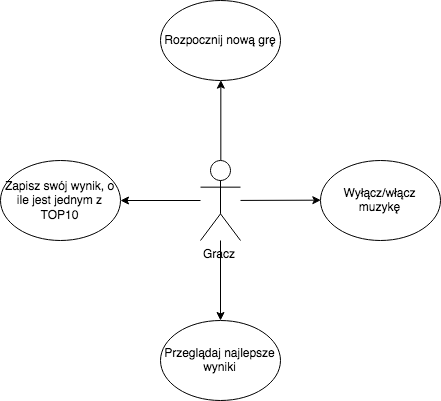
\includegraphics[scale=0.5]{use_case_diagram.png}
\end{center}

\subsection{Opis wybranych przypadków użycia}

\subsubsection{Gra}

\begin{enumerate}
    \item Gracz wybiera przycisk 'Rozpocznij nową grę'.
    \item Aplikacja wyświetla ekran z grą.
    \item Gracz gra w grę kładąc kolejne klocki.
    \item Gracz kończy grę nietrafiając klockiem w podstawę poprzeniego.
    \item Jeżeli wynik gracza jest jednym z 10 najlepszych, gracz zapisuje wynik.
\end{enumerate}

\subsubsection{Najlepsze wyniki}
\begin{enumerate}
    \item Gracz wybiera przycisk 'TOP 10'.
    \item Aplikacja wyświetla ekran z listą co najwyżej 10 najlepszych wyników.
\end{enumerate}

\section{Wymagania niefunkcjonalne}

\end{document}
